\section{Photodiode}

Solid state detectors like the photodiode are based on the properties of semiconductors. These types of detectors have marked advantages over other types of detectors, they can be kept smaller than gas-filled detectors due to their density and also have better energy resolution than the scintillator counters \cite[Chap 11.]{knollRadiationDetectionMeasurement2010}. In this section, we will discuss the basic concepts of semiconductors and how they can be used as detectors.

\subsection{Semiconductors}
\subsubsection{Band Structure and Charge Carriers}

In crystalline solid materials, the periodic lattice structures restrict electron energies to distinct allowed bands that are separated by forbidden energies as shown in the diagram \cref{fig:band_structure}. The lower of these energy regions, known as the valence band, contains outer-shell electrons that are placed in a specific position inside the lattice via interatomic bonds. Conversely, the higher-lying conduction band represents free electrons capable of migrating through the crystal lattice and this electrons allow  electrical conductivity to be present. The magnitude of the forbidden energy gap or bandgap between these two bands dictates whether a material functions as an insulator or a semiconductor. 

In the absence of thermal excitation, both insulators and semiconductors maintain a completely filled valence band and a completely empty conduction band, resulting in no electrical conductivity under these baseline conditions. In contrast, metals feature not entirely filled highest energy band, permitting electrons to easily migrate within the crystal lattice with minimal incremental energy and thus ensuring high electrical conductivity across the material. For insulators and semiconductors, however, electrons must first cross the intervening bandgap to reach the conduction band, causing their baseline electrical conductivity to be many orders of magnitude lower \cite[Chap 11.]{knollRadiationDetectionMeasurement2010}.

\begin{figure}[htbp]
    \centering
    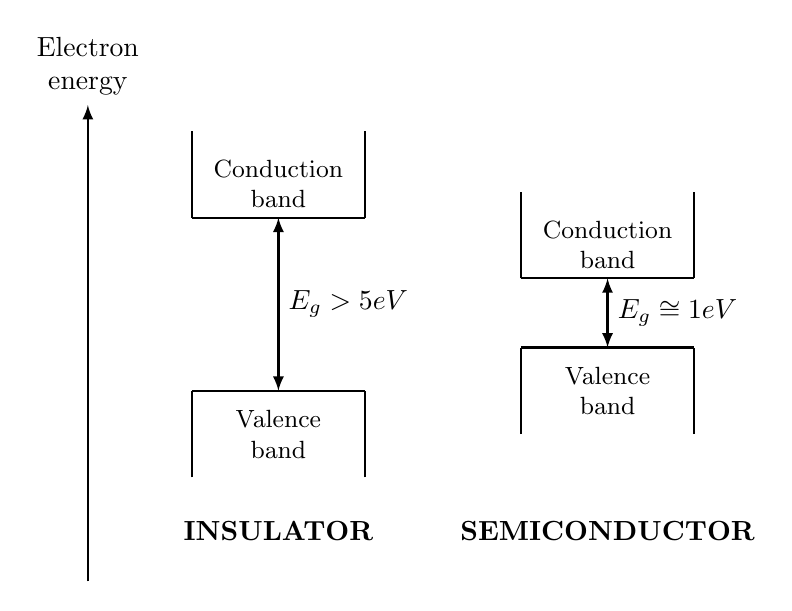
\begin{tikzpicture}[scale=1.1, >=latex]
        % Eje de energía vertical
        \draw[->, thick] (0,0) -- (0,5.5) node[above, align=center] {Electron\\energy};

        % --- AISLANTE (INSULATOR) ---
        \begin{scope}[shift={(1.2,0)}]
            % Banda de conducción
            \draw[thick] (0,4.2) -- (2.0,4.2);
            \node[above, align=center, font=\small] at (1.0,4.2) {Conduction\\band};
            \draw[thick] (0,4.2) -- (0,5.2);
            \draw[thick] (2.0,4.2) -- (2.0,5.2);

            % Flecha de banda prohibida (Eg > 5 eV)
            \draw[<->, thick] (1.0,2.2) -- node[right, align=left] {$E_g > 5\text{ eV}$} (1.0,4.2);

            % Banda de valencia
            \draw[thick] (0,2.2) -- (2.0,2.2);
            \draw[thick] (0,1.2) -- (0,2.2);
            \draw[thick] (2.0,1.2) -- (2.0,2.2);
            \node[align=center, font=\small] at (1.0, 1.7) {Valence\\band};

            % Etiqueta inferior
            \node[below, font=\bfseries] at (1.0, 0.8) {INSULATOR};
        \end{scope}

        % --- SEMICONDUCTOR ---
        \begin{scope}[shift={(5.0,0)}]
            % Banda de conducción
            \draw[thick] (0,3.5) -- (2.0,3.5);
            \node[above, align=center, font=\small] at (1.0,3.5) {Conduction\\band};
            \draw[thick] (0,3.5) -- (0,4.5);
            \draw[thick] (2.0,3.5) -- (2.0,4.5);

            % Flecha de banda prohibida (Eg ≈ 1 eV)
            \draw[<->, thick] (1.0,2.7) -- node[right, align=left] {$E_g \cong 1\text{ eV}$} (1.0,3.5);

            % Banda de valencia
            \draw[thick] (0,2.7) -- (2.0,2.7);
            \draw[thick] (0,1.7) -- (0,2.7);
            \draw[thick] (2.0,1.7) -- (2.0,2.7);
            \node[align=center, font=\small] at (1.0, 2.2) {Valence\\band};

            % Etiqueta inferior
            \node[below, font=\bfseries] at (1.0, 0.8) {SEMICONDUCTOR};
        \end{scope}

    \end{tikzpicture}
    \caption{Band structure for electron energies in insulators and semiconductors \cite[Chap 11.]{knollRadiationDetectionMeasurement2010}.}
    \label{fig:band_structure}
\end{figure}

At any temperature greater than zero the thermal energy introduced into the electrons within the lattice allows them to gain sufficient energy to cross the bandgap into the conduction band, leaving behind a vacancy known as a hole. This combination forms an electron-hole pair. Under the influence of an applied electric field, conduction electrons migrate toward positive potentials while positive holes move in the opposite direction, with the motion of both charge carriers contributing directly to the material's observed electrical conductivity. 

\begin{equation}
    p(T) = C T^{3/2} \exp\left(-\frac{E_g}{2kT}\right)
    \label{eq:thermal_generation}
\end{equation}

where:
\begin{itemize}
    \item $T =$ absolute temperature
    \item $E_g =$ bandgap energy
    \item $k =$ Boltzmann constant
    \item $C =$ proportionality constant characteristic of the material
\end{itemize}

The probability per unit time for thermal electron-hole pair generation is given by \cref{eq:thermal_generation} in \cite[p. 367]{knollRadiationDetectionMeasurement2010}. This generation of electron-hole pairs is heavily dependent on the ratio of the bandgap energy to the absolute temperature of the material. Consequently, materials with bigger bandgaps experience minimal thermal excitation that could create conductivity and thus act as insulators, while materials with smaller bandgaps yield sufficient conductivity to be classified as semiconductors. When there is no electric field pulling them apart, the electrons and holes created by heat eventually find each other and recombine canceling each other out. They constantly form and recombine until they reach a stable balance, this balance depends heavily on heat. If the material is cooled down, there is less thermal energy available, causing the number of active electron-hole pairs to drop drastically.


\subsubsection{Effect of Impurities of Dopants}



\subsubsection{Action of Ionizing Radiation on Semiconductors}

\subsection{Semiconductors as Detectors}

\subsubsection{Photodiodes as Detectors}


\todo[inline]{photodiode working}

\subsection{Integration on the setup}
\todo[inline]{photos and setup of the 3d printed support and the photodiode with the interferometer  and the circuit used to convert the current into voltage.}